\clearpage
\section{Technische Grundlagen Bluetooth Mesh}\label{sec:TechnischeGrundlagenBluetoothMesh}




\subsection{Netzaufbau und Topologie}\label{sec:NetzaufbauundTopologie}

Nebst dem Funktionellen Aspekt übernehmen Nodes unterschiedliche Rollen im Netzaufbau. Ein Node wird als Relay-Node bezeichnet wenn dieser Nachrichten an weitere Teilnehmer weiterleitet. Ein Friend-Node dient als Zugangspunkt für einen Low-Power-Node. Der Low-Power-Node wird dort eingesetzt wo keine konstante Stromversorgung zur Verfügung steht. Dieser geht in eine Beziehung mit einem Friend-Node, welcher alle Nachrichten für diesen zwischenspeichert. Über ein Zeitintervall fragt dieser die verpassten Nachrichten beim Friend ab. Dadurch kann der LPN zwischen Abfragen inaktiv sein um Energie zu sparen. Um die Interoperabilität zwischen inkompatiblen Bluetooth-Mesh Geräten und einem Mesh-Netzwerk zu ermöglichen existieren Proxy-Nodes. Ein Proxy-Node dient als Schnittstelle in das Netzwerk und erlaubt das Interagieren über Bluetooth-GATT mit dem Mesh. Die in Abbildung \ref{fig:BTMeshTopology} gezeigt Topologie zeigt die verschiedenen Node-Typen an ihrem Einsatzort. 

\begin{figure} [H]
	\centering
	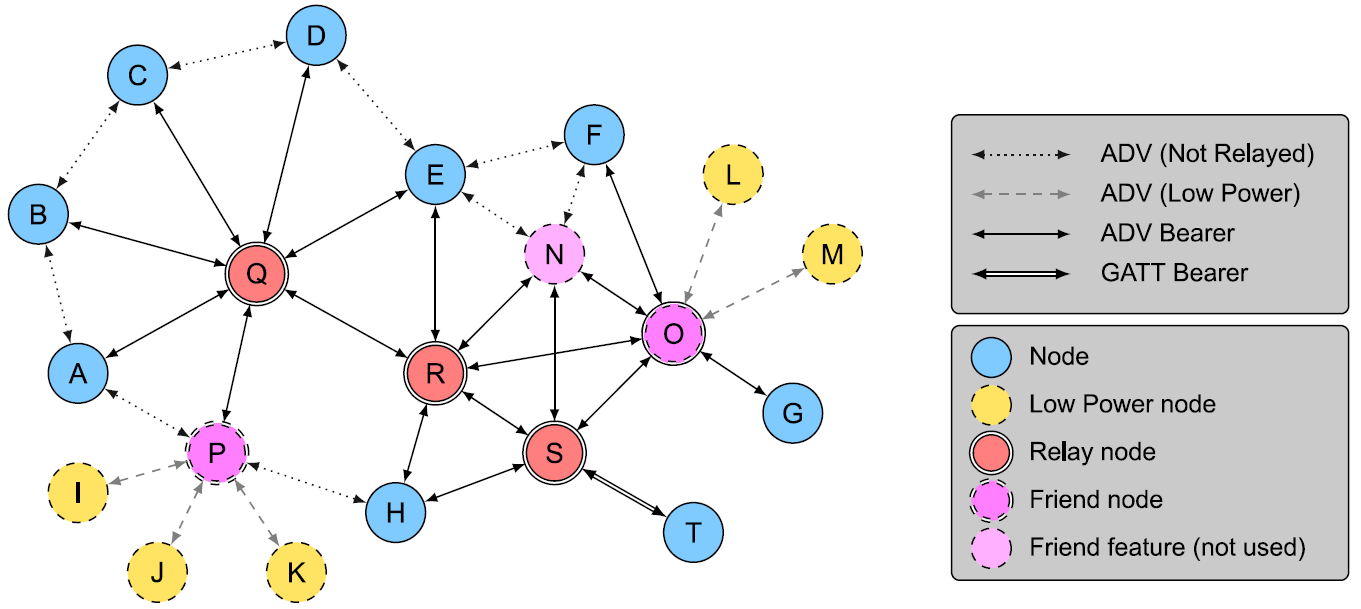
\includegraphics[width=1.0\textwidth]{Bluetooth_Mesh_Topology.PNG}
	\caption{Topologie eines Bluetooth-Mesh Netzwerks \cite{bluetooth_sig_mesh_netzwerk_spezifikationen_2020}} 
	\label{fig:BTMeshTopology}
\end{figure}





\todo[inline]{Welchen Aufbau? Welche Art von Mesh? Welche Nodetypen gibt es? Welche typischen Eigenschaften besitzt das Protokoll?}

\subsection{Bluetooth Mesh Protokoll Stack}\label{sec:ZigbeeProtokollStack}

In diesem Abschnitt wird die Architektur des Mesh-Stacks genauer untersucht. Wie in Kapitel \ref{sec:EinleitungBluetooth} bereits erwähnt basiert der Stack auf Bluetooth Low Energy. Der BLE-Layer dient zur Grundlegenden Schicht des Stacks. 

\begin{figure} [H]
	\centering
	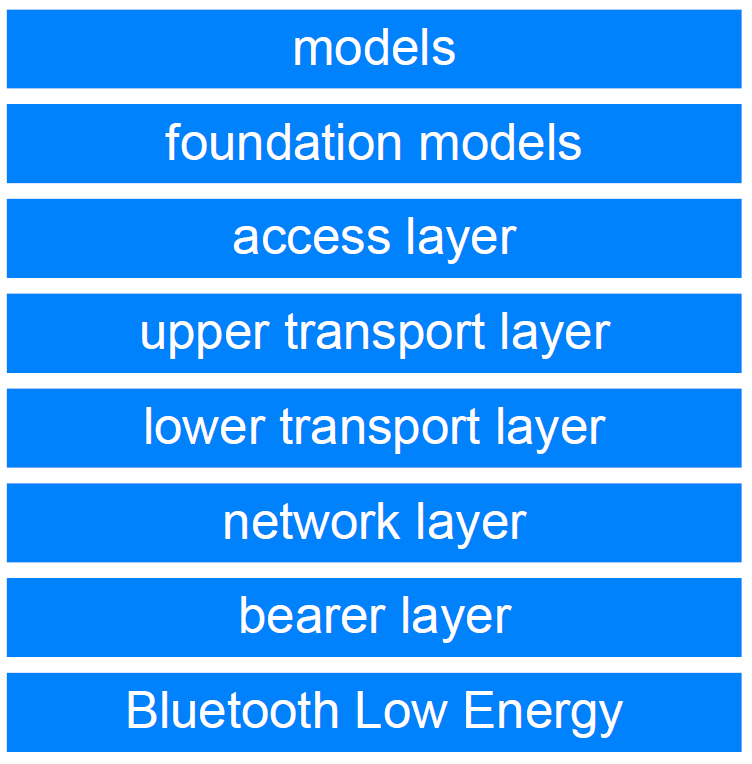
\includegraphics[width=0.5\textwidth]{Bluetooth_Mesh_Stack_Layers.PNG}
	\caption{Bluetooth-Mesh Stack \cite{bluetooth_sig_mesh-technology-overviewpdf_2020}} 
	\label{fig:BTMeshStack}
\end{figure}

\todo[inline]{Erläuterung des Protokoll Stacks. Möglichst viel Grafiken und nur so viel als nötig Prosa.}

\subsection{Bluetooth Mesh Software Development Kit}\label{sec:ZigbeeSoftwareDevelopmentKit}
\todo[inline]{Eingesetzte SDK und deren Aufbau beschreiben. Allenfalls die wichtigsten API Funktionen genauer erläutern.}


